\section{Introduction}
\label{introduction}


\subsection{Single Object Tracking}

Single object tracking is essentially a filtering problem. We are dealing with sequential processing of a noisy
sensor measurements in order to determine the state of the object.

\begin{framed}
\begin{remark}{}

When we say state we actually mean the position of the object together with properties that describe
its motion e.g. speed and direction
\end{remark}
\end{framed}

The filtering problem is not so easy to solve since the state of the object is neither fully not directly observed.


\begin{framed}
\begin{definition}{\textbf{Multiple Object Tracking (MOT)}}

Multiple Object Tracking is defined as the sequentioal processing of noisy sensor measurements in order to determine
the number of dynamic objects in each dynamic state of the object.  
\end{definition}
\end{framed}


Typically MOT is based on sensor detections. common sensors in MOT are

\begin{itemize}
\item Cameras
\item Radars
\item LiDARs
\end{itemize}

In addition, the sensor data serves as input to a detector. The block diagram in Figure \ref{sensor_mot_block_diagram} illustrates the concept.

\begin{figure}[!htb]
\begin{center}
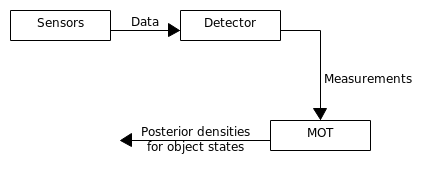
\includegraphics[scale=0.480]{img/object_tracking/sensor_mot_block_diagram.png}
\end{center}
\caption{MOT block diagram.}
\label{sensor_mot_block_diagram}
\end{figure}

\begin{figure}[!htb]
\begin{center}
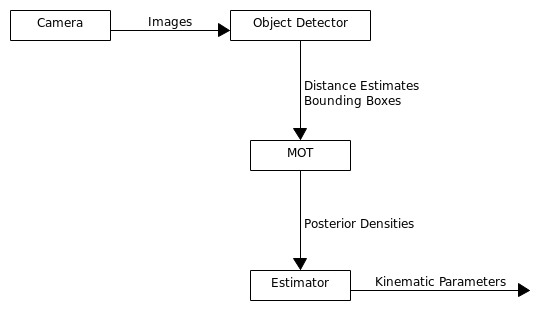
\includegraphics[scale=0.480]{img/object_tracking/camera_block_diagram.png}
\end{center}
\caption{Camera block diagram.}
\label{camera_block_diagram}
\end{figure}

\subsection{Questions}

\begin{enumerate}
\item Which property or properties hold(s) for the track-before-detect method?
\item Which property or properties hold(s) for the point object tracking method?
\item Which property or properties hold(s) for the extended object tracking method?
\item Which property or properties hold(s) for the group object tracking method?
\item Which property or properties hold(s) for the tracking with multi-path propagation method?
\item Which property or properties hold(s) for the tracking with unresolved measurements method?
\end{enumerate}

\subsection{Assignements}
